\section{Evaluation}
\label{sec:evaluation}

% Results figures, rendered from the persisted artifacts:
% bootstrap_ci.json (suite means and 95% CIs), stability_run1_vs_run2.json (run pairs).
% Values resolve through figures/generated_values.tex, which scripts/gen_sp_figures.py
% writes from those artifacts; run `python scripts/gen_sp_figures.py --check` to prove
% this figure still agrees with them.
% Layout discipline: the top panel shows point estimates + intervals only
% (no filled bars under the whiskers), the bottom panel's legend lives
% below the axis (never over the bars), and both panels share the same
% value range so the stacked scales read as one.
% GENERATED by scripts/gen_sp_figures.py -- do not edit by hand.
% Every plotted number in the S&P figures resolves through this file, so a
% figure cannot silently disagree with the artifact it claims to show.
% Regenerate:  python scripts/gen_sp_figures.py
% Verify:      python scripts/gen_sp_figures.py --check
% Sources:
%   results/bootstrap_ci.json
%   results/stability_run1_vs_run2.json
%   results/b4_baseline_zodiac_20260922.json
%   results/model_quality/chrollo_calibration.json
%   results/sp2027_rescue/behavior_trajectory_benchmark.json

\def\RaginLiveTechnique{0.9598}
\def\RaginLiveTechniqueErrLo{0.0122}
\def\RaginLiveTechniqueErrHi{0.0122}
\def\RaginLiveActor{0.8500}
\def\RaginLiveActorErrLo{0.0000}
\def\RaginLiveActorErrHi{0.0000}
\def\RaginLivePersona{0.7325}
\def\RaginLivePersonaErrLo{0.0587}
\def\RaginLivePersonaErrHi{0.0558}
\def\RaginLiveComposite{0.8796}
\def\RaginLiveCompositeErrLo{0.0224}
\def\RaginLiveCompositeErrHi{0.0204}
\def\RaginLivePersonaRunTwo{0.7504}
\def\RaginLiveCompositeRunTwo{0.8845}
\def\RaginPersonaRunDelta{0.018}
\def\RaginTechDelta{0.317}
\def\RaginTechDeltaLo{0.162}
\def\RaginTechDeltaHi{0.480}
\def\RaginActorDelta{0.140}
\def\RaginActorDeltaLo{0.083}
\def\RaginActorDeltaHi{0.197}
\def\RaginPersonaNullDelta{0.005}
\def\RaginPersonaNullDeltaLo{-0.047}
\def\RaginPersonaNullDeltaHi{0.057}
\def\RaginOverallDelta{0.154}
\def\RaginOverallDeltaLo{0.092}
\def\RaginOverallDeltaHi{0.221}
\def\RaginGroundingTtpCount{35}
\def\RaginNoGroundingTtpCount{0}
\def\RaginRoutingBefore{0.8875}
\def\RaginRoutingAfter{0.955}

\begin{figure}[t]
\centering
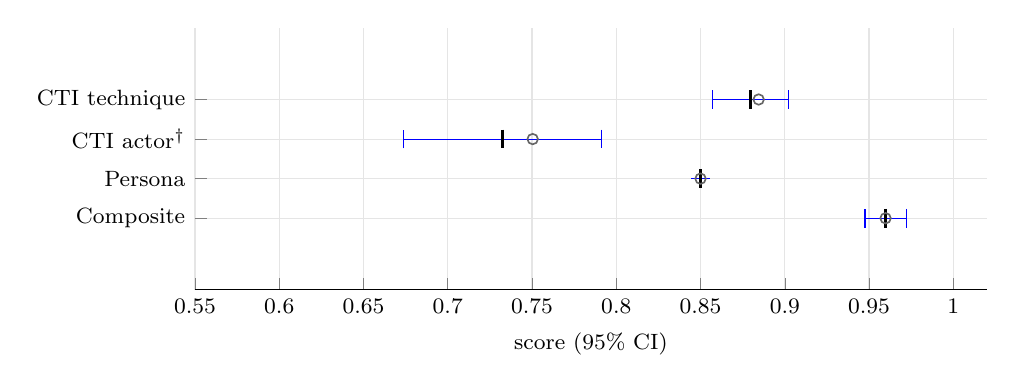
\begin{tikzpicture}
\begin{axis}[
  name=ax1,
  width=0.96\linewidth,
  height=4.9cm,
  xmin=0.55, xmax=1.02,
  y axis line style={draw=none},
  axis x line*=bottom,
  axis y line*=left,
  ytick=data,
  yticklabels={Composite,Persona,CTI actor$^{\dagger}$,CTI technique},
  y dir=reverse,
  xlabel={score (95\% CI)},
  xlabel style={font=\footnotesize},
  tick label style={font=\footnotesize},
  enlarge y limits=0.6,
  grid=major,
  grid style={black!10},
  clip=false
]
% point estimates and bootstrap 95% CIs from bootstrap_ci.json;
% only marks + intervals: no bars beneath the whiskers
\addplot+[only marks, mark=|, mark size=3.4, mark options={thick,black},
  error bars/.cd, x dir=both, x explicit] coordinates {
  (\RaginLiveTechnique,3) +- (\RaginLiveTechniqueErrLo,\RaginLiveTechniqueErrHi)
  (\RaginLiveActor,2) +- (\RaginLiveActorErrLo,\RaginLiveActorErrHi)
  (\RaginLivePersona,1) +- (\RaginLivePersonaErrLo,\RaginLivePersonaErrHi)
  (\RaginLiveComposite,0) +- (\RaginLiveCompositeErrLo,\RaginLiveCompositeErrHi)
};
% run-2 overlay: open markers (point estimates from stability_run1_vs_run2.json;
% per-suite CIs were not computed for run 2, so none are drawn)
\addplot+[only marks, mark=o, mark size=1.9, mark options={semithick,black!60}] coordinates {
  (\RaginLiveTechnique,3)
  (\RaginLiveActor,2)
  (\RaginLivePersonaRunTwo,1)
  (\RaginLiveCompositeRunTwo,0)
};
\end{axis}
\end{tikzpicture}

\vspace{2mm}

\begin{tikzpicture}
\begin{axis}[
  name=ax2,
  width=0.96\linewidth,
  height=4.9cm,
  ybar=1.5pt,
  bar width=9pt,
  ymin=0.55, ymax=1.0,
  symbolic x coords={CTI technique,CTI actor,Persona,Composite},
  xtick=data,
  ylabel={mean score},
  ylabel style={font=\footnotesize},
  tick label style={font=\footnotesize},
  ymajorgrids,
  grid style={black!10},
  enlarge x limits=0.25,
  legend style={font=\scriptsize, at={(0.5,-0.16)}, anchor=north, legend columns=2, draw=none, fill=none},
  legend cell align={left},
]
% run 1 vs run 2 from stability_run1_vs_run2.json
\addplot+[black!35, fill=black!35] coordinates {
  (CTI technique,\RaginLiveTechnique) (CTI actor,\RaginLiveActor) (Persona,\RaginLivePersona) (Composite,\RaginLiveComposite)
};
\addplot+[black!70, fill=black!70, pattern=north east lines] coordinates {
  (CTI technique,\RaginLiveTechnique) (CTI actor,\RaginLiveActor) (Persona,\RaginLivePersonaRunTwo) (Composite,\RaginLiveCompositeRunTwo)
};
\legend{run 1, run 2}
\end{axis}
\end{tikzpicture}
\caption{Live-campaign results from the persisted artifacts (identical
deterministic-strata bars across runs are the finding, not a plotting
error). All four plotted values are the \emph{both-channel} operational
score of Table~\ref{tab:live}, which fuses the served-text and CTI-analysis
channels; they are not served-quality results, and the echo-guarded bounds
for the same rows are 0.479 technique and 0.243 actor.
\emph{Top:}
suite means with bootstrap 95\% confidence intervals; open markers mark
the independent second run's point estimates, and the actor interval is
degenerate ($^{\dagger}$) because the actor rubric assigns the same
score to every row, so uncertainty is carried by the Wilson pass-rate
interval instead (Table~\ref{tab:live}). \emph{Bottom:} two independent
218-query campaigns; the deterministic CTI strata replicate exactly and
only the LLM-judged persona stratum moves, by $+\RaginPersonaRunDelta$.}
\label{fig:results}
\end{figure}


We evaluate the loop as a serving system, separating what the attacker
receives (the \emph{served-text} channel) from what the retrieval pipeline
identifies for the operator (the \emph{CTI-analysis} channel). The latter is
never served. All headline results are backed by persisted JSON or JSONL
artifacts. Paired grounding differences use a 10,000-resample percentile
bootstrap over scenario-level differences. The induced-draft battery instead
resamples whole \emph{cases} (cluster bootstrap, 10,000 iterations, unit =
case), because the repeats inside a case share one scenario and are not
independent; its intervals are therefore wider than the draft-level binomial
intervals they replace, and the draft-level ones are not used. The
deterministic suites carry exactly one draft per case, so clustering is
vacuous there and their intervals are binomial over cases.

\subsection{Setup and Grounding}
\label{sec:setup}
The archived runs execute against a 2-vCPU, ${\sim}4$-GB single-host
deployment; the evaluation harness runs on a separate workstation and shares
no state with the deployed stack. The fixed
workload contains 123 CTI-technique queries, 35 CTI-actor queries, and 60
persona sessions. The generator and judge use different model families from
one free-tier provider; catalog drift, quota exhaustion, gateway outages, and
alignment refusals are absorbed by the deterministic floor. Fresh
provider-backed reruns are currently unavailable. The paired grounding
experiment runs 30 scenarios in each of the technique, actor, and persona
strata with identical prompts and retrieval removed only in the control arm.
Because that design is balanced across strata while the live workload is not,
the ablation estimates a balanced-stratum mean difference rather than the
deployment-weighted composite of Table~\ref{tab:live}; the two are not the
same estimand, and no correction is applied across the three strata and the
pooled row because each interval is already far from its null.

Table~\ref{tab:provenance} records which generator produced which surface.
The surfaces were not produced by one model, so results are not compared
across them; the version-of-record campaign predates the model pin and its
generator was not logged.

\begin{table*}[t]
\centering
\caption{Generator provenance per measured surface. The campaign, the ladder,
and the scorer audit were produced by three different generators; no number is
compared across rows.}
\label{tab:provenance}
\scriptsize
\setlength{\tabcolsep}{5pt}
\begin{tabular}{p{0.33\textwidth}>{\raggedright\arraybackslash}p{0.60\textwidth}}
\toprule
Surface & Generator / gateway \\
\midrule
Paired grounding ablation (Table~\ref{tab:b4})
  & not logged (pre-pin gateway default) \\
Version-of-record campaign (Table~\ref{tab:live})
  & not logged (pre-pin gateway default) \\
Same-model ladder (Table~\ref{tab:baseline-served-text})
  & \texttt{deepseek-v4-flash-free} on \texttt{api.apmix.ai} \\
Scorer-validity audit corpus (\S\ref{sec:scorer-audit})
  & gateway default (\texttt{glm-5.3-flash-free}) \\
Induced-draft battery (Table~\ref{tab:verifier-cross-family})
  & \texttt{space-bunny-free}, \texttt{deepseek-v4-flash-free} on
    \texttt{api.apmix.ai}; \texttt{llama-3.3-70b-instruct} on
    \texttt{openrouter.ai} \\
Deception-quality judge (\S\ref{sec:rq3})
  & one judge model, same provider as the generator \\
\bottomrule
\end{tabular}
\end{table*}

\begin{table}[t]
\centering
\caption{Paired grounding ablation: 90 matched scenario pairs. Scores are
the declared analysis-channel composite; channel attribution follows the
recorded scorer configuration and measurement lineage, as the archived
artifact carries no channel field. CIs are paired bootstrap intervals.
The archived artifact pairs by scenario name; new reruns must persist canonical
scenario IDs and manifest hashes.}
\label{tab:b4}
\scriptsize
\setlength{\tabcolsep}{3.5pt}
\begin{tabular}{lccc}
\toprule
Suite & RAG & No-RAG & Difference (95\% CI) \\
\midrule
Technique & 0.950 & 0.633 & $+0.317$ $[+0.162,+0.480]$ \\
Actor & 0.850 & 0.710 & $+0.140$ $[+0.083,+0.197]$ \\
Persona & 0.833 & 0.828 & $+0.005$ $[-0.047,+0.057]$ \\
\midrule
Overall & & & $+0.154$ $[+0.092,+0.221]$ \\
\bottomrule
\end{tabular}
\end{table}

% Paired grounding effect (RAG minus No-RAG) per suite with 95% bootstrap
% CIs, from b4_baseline_zodiac_20260922.json (the same numbers as
% Table~tab:b4). Filled markers: intervals excluding zero. Open marker:
% the persona stratum, whose interval straddles zero exactly as the
% architecture predicts. Compiled statically; no results directory needed.
% GENERATED by scripts/gen_sp_figures.py -- do not edit by hand.
% Every plotted number in the S&P figures resolves through this file, so a
% figure cannot silently disagree with the artifact it claims to show.
% Regenerate:  python scripts/gen_sp_figures.py
% Verify:      python scripts/gen_sp_figures.py --check
% Sources:
%   results/bootstrap_ci.json
%   results/stability_run1_vs_run2.json
%   results/b4_baseline_zodiac_20260922.json
%   results/model_quality/chrollo_calibration.json
%   results/sp2027_rescue/behavior_trajectory_benchmark.json

\def\RaginLiveTechnique{0.9598}
\def\RaginLiveTechniqueErrLo{0.0122}
\def\RaginLiveTechniqueErrHi{0.0122}
\def\RaginLiveActor{0.8500}
\def\RaginLiveActorErrLo{0.0000}
\def\RaginLiveActorErrHi{0.0000}
\def\RaginLivePersona{0.7325}
\def\RaginLivePersonaErrLo{0.0587}
\def\RaginLivePersonaErrHi{0.0558}
\def\RaginLiveComposite{0.8796}
\def\RaginLiveCompositeErrLo{0.0224}
\def\RaginLiveCompositeErrHi{0.0204}
\def\RaginLivePersonaRunTwo{0.7504}
\def\RaginLiveCompositeRunTwo{0.8845}
\def\RaginPersonaRunDelta{0.018}
\def\RaginTechDelta{0.317}
\def\RaginTechDeltaLo{0.162}
\def\RaginTechDeltaHi{0.480}
\def\RaginActorDelta{0.140}
\def\RaginActorDeltaLo{0.083}
\def\RaginActorDeltaHi{0.197}
\def\RaginPersonaNullDelta{0.005}
\def\RaginPersonaNullDeltaLo{-0.047}
\def\RaginPersonaNullDeltaHi{0.057}
\def\RaginOverallDelta{0.154}
\def\RaginOverallDeltaLo{0.092}
\def\RaginOverallDeltaHi{0.221}
\def\RaginGroundingTtpCount{35}
\def\RaginNoGroundingTtpCount{0}
\def\RaginRoutingBefore{0.8875}
\def\RaginRoutingAfter{0.955}

\begin{figure}[t]
\centering
\begin{tikzpicture}[
  font=\scriptsize,
  dot/.style={circle, fill=black, inner sep=1.5pt},
  nul/.style={circle, draw=black, fill=white, inner sep=1.5pt, thick},
  arr/.style={-{Latex[length=1.6mm]}, semithick, black!55}
]
  % zero reference
  \draw[black!45] (0,0.5) -- (0,-3.2);
  \node[font=\tiny, text=black!60, anchor=east] at (-0.05,0.5) {$\Delta=0$};

  % CTI technique: +0.317 [+0.162, +0.480]
  \node[anchor=east] at (-0.25,0) {CTI technique};
  \draw[black!70] (1.62,0) -- (4.80,0);
  \draw[black!70] (1.62,-0.13) -- (1.62,0.13);
  \draw[black!70] (4.80,-0.13) -- (4.80,0.13);
  \node[dot] at (3.17,0) {};

  % CTI actor: +0.140 [+0.083, +0.197]
  \node[anchor=east] at (-0.25,-0.95) {CTI actor};
  \draw[black!70] (0.83,-0.95) -- (1.97,-0.95);
  \draw[black!70] (0.83,-1.08) -- (0.83,-0.82);
  \draw[black!70] (1.97,-1.08) -- (1.97,-0.82);
  \node[dot] at (1.40,-0.95) {};

  % Persona (predicted null): +0.005 [-0.047, +0.057]
  \node[anchor=east] at (-0.25,-1.9) {Persona};
  \draw[black!70] (-0.47,-1.9) -- (0.57,-1.9);
  \draw[black!70] (-0.47,-2.03) -- (-0.47,-1.77);
  \draw[black!70] (0.57,-2.03) -- (0.57,-1.77);
  \node[nul] at (0.05,-1.9) {};

  % Overall
  \draw[black!25, dashed] (-0.25,-2.5) -- (5.0,-2.5);
  \node[anchor=east] at (-0.25,-3.0) {Overall (90 pairs)};
  \draw[black!70] (0.92,-3.0) -- (2.21,-3.0);
  \draw[black!70] (0.92,-3.13) -- (0.92,-2.87);
  \draw[black!70] (2.21,-3.13) -- (2.21,-2.87);
  \node[dot] at (1.54,-3.0) {};

  % axis
  \draw[arr] (0,-3.65) -- (5.1,-3.65);
  \foreach \x/\l in {0/0, 1/{+0.1}, 2/{+0.2}, 3/{+0.3}, 4/{+0.4}} {
    \draw[black!55] (\x,-3.58) -- (\x,-3.72)
        node[below, font=\tiny, text=black!60] {\l};
  }
\end{tikzpicture}
\caption{Paired grounding differential (RAG $-$ No-RAG) per suite with
95\% bootstrap CIs over 90 scenario pairs (numbers in
Table~\ref{tab:b4}). Filled markers: intervals excluding zero -- $+\RaginTechDelta$
on technique detection and $+\RaginActorDelta$ on actor attribution. The open
marker is the persona stratum, whose interval straddles zero exactly as
the architecture predicts: host believability is produced by the
deception engine and the fiction graph, not by threat-intelligence
retrieval. The mechanism behind the technique effect is starker than
the mean: the grounded arm yields \RaginGroundingTtpCount{} TTP detections spanning 21 distinct
techniques, while the ungrounded arm yields none.}
\label{fig:grounding}
\end{figure}


The analysis channel detects 35 TTPs spanning 21 techniques versus zero
without retrieval, while persona realism remains unchanged. The null is informative:
host believability is produced by the fiction graph and deception engine,
whereas CTI intelligence is the retrieval-dependent capability. The full
grounded campaign records 132 detections spanning 67 unique techniques.

\subsection{Serving Safety and Induced Failures}
\label{sec:rq2}
The live workload records zero contradictions across 45 targeted re-queries,
zero pinned-identity violations, and zero serves after a failed verifier
verdict. In the 218-query campaign, 218 sessions engage and 218 persona
assignments are correct; the declared both-channel composite is 0.880, which
Table~\ref{tab:live} reports beside its echo-guarded bound rather than as a
standalone capability score.

Serve-path provenance is taken from the per-serve labels the pipeline stamps,
not from response time: the archived tally records 216 of 218 responses as
\texttt{GENERATED\_VERIFIED} and 2 as \texttt{FALLBACK\_VERIFIED}, with no
serve labeled as a fail-safe substitution. A later scorer-validity audit
found that gateway-outage and template-anchored serves had carried no marker
in that tally and were counted as verified generation; they are now stamped
\texttt{TEMPLATE\_FALLBACK\_VERIFIED}, and roughly one hundred rows on the
CTI surface serve template-echoed text. A latency-based cross-check that
classifies any turn faster than $4\,\mathrm{s}$ as vetted deterministic
content estimates an $88.1/11.9$ split --- a lower bound on the deterministic
share rather than an audited count. One disclosure bounds the
zero-contradiction claim: 11.9\% of serves are estimated deterministic-path,
so some of the 45 re-queries may be template serves for which consistency is
a property of the vetted library rather than graph-enforced generation. A
serve-path-stamped re-run remains future work; the zero-contradiction result
itself is unaffected, since both serve paths are verified or vetted by
construction.

\begin{table}[t]
\centering
\caption{Version-of-record 218-row campaign. Column~3 is the declared
\emph{both-channel} operational score, which fuses the served-text and
CTI-analysis channels and therefore is not a served-quality result. Column~4
is the echo-guarded lower bound computed on these same archived rows, where
template-echo rows are zeroed and the remainder keeps its both-channel score;
because the stored responses are truncated previews, column~4 is a lower
bound and not the guarded served-text mean.}
\label{tab:live}
\scriptsize
\setlength{\tabcolsep}{4pt}
\begin{tabular}{lrrr}
\toprule
Suite & $n$ & Both-channel & Guarded LB \\
\midrule
Technique & 123 & 0.960 & 0.479 \\
Actor & 35 & 0.850 & 0.243 \\
Persona & 60 & 0.733 & 0.733 \\
\midrule
Composite & 218 & 0.880 & 0.511 \\
\bottomrule
\end{tabular}
\end{table}

\begin{table}[t]
\centering
\caption{Verifier stress test after the P1 extraction fixes. Live rows are
authored drafts, not served sessions; the llama row includes 48 disclosed
substitute-author fills. Intervals are 95\% cluster bootstraps that resample
cases (89, 80, and 94 cases; 105 for the deterministic suite, which carries one
draft per case). Bootstrapping cases rather than drafts widens the llama
precision interval from $[.869,.947]$ to $[.858,.962]$.}
\label{tab:verifier-cross-family}
\scriptsize
\setlength{\tabcolsep}{2.5pt}
\begin{tabular}{lrrrrr}
\toprule
Author & Drafts & P & 95\% CI & R & 95\% CI \\
\midrule
space-bunny-free & 261 & 1.000 & $[1.000,1.000]$ & 0.959 & $[.926,.985]$ \\
deepseek-v4-flash-free & 236 & 1.000 & $[1.000,1.000]$ & 0.983 & $[.961,1.000]$ \\
llama-3.3-70b & 281 & 0.916 & $[.858,.962]$ & 0.898 & $[.848,.943]$ \\
\midrule
Pooled (778 drafts) & 778 & 0.970 & $[.949,.987]$ & 0.944 & $[.922,.965]$ \\
Canonical deterministic & 105 & 1.000 & -- & 1.000 & -- \\
\bottomrule
\end{tabular}
\end{table}

The clean workload tests the deployed serving invariant, not sensitivity to
bad drafts. The canonical 105-case suite has 78 reject and 27 pass cases and
achieves perfect precision and recall on danger, identity, consistency, and
degenerate checks. The cross-family matrix induces failures and exposes the
real boundary: post-fix recall is 0.898--0.983 and precision is
0.916--1.000. Residual errors concentrate in author-side identity drift and
model-specific tell vocabulary. Thus the paper claims fail-closed serving,
not universal semantic coverage.

\paragraph{What the gate prevented.}
The clean campaign does not exercise the gate. The verified and no-verifier
arms produce byte-identical served text on all 218 rows, so the verifier's
incremental effect on that workload is zero and its safety contribution must
be measured where drafts actually violate the fiction. Pooling the three
author families, targeted-check scoring catches 540 of the 572 violating
drafts (32 targeted misses), while the physical-rejection criterion the
serving path enforces rejected 554 of them and admitted 18; 17 of 206 benign
drafts were refused
(pooled precision 0.970 $[.949,.987]$, recall 0.944 $[.922,.965]$, cluster
bootstraps that resample cases within each author family). The one fully
attributed family (llama-3.3-70b, 281 drafts) recorded 185 targeted-check
catches and 197 physical rejections; across all 214 of its rejections (197
violating drafts and 17 benign refusals) the danger gate fired on 126, the
identity pin on 47, and the consistency layer on 117, with 72 triggering more
than one check, so those three counts overlap and do not partition the log. Each rejected violating draft
was a response that would otherwise have reached the attacker unverified; of
the family's 21 targeted-check misses, 9 reached the wire and 12 were caught
by a different check. Both prompt-injection cases in that battery carry
targeted-scoring misses, and one variant of one case passed the gate;
Section~\ref{sec:threat-model} therefore withdraws injection coverage from
the property table.

\paragraph{Where the gate's coverage ends.}
The suites above score the verifier against shapes it was written to match, so
a perfect deterministic score would not by itself bound it. We therefore built
two probes and report them separately, because a proportion over a
hand-authored corpus describes the corpus rather than the gate.

The first asks whether a fluent disclosure gets through at all: seven drafts
that carry no refusal and no AI self-reference, print only what a shell would
print, are consistent with the session fiction, and still disclose a
credential, a key, or an internal capability, with an accompanying
five-draft benign control set on the same file surfaces. The gate stopped four of the seven---a
plaintext application credential and a bearer-token dotenv file by the danger
gate, a leaked persona configuration by the danger gate, and an
internal-topology dump by the consistency layer---and refused none of the five
benign drafts. The three that reached the wire were a PEM private key in a
format no registered secret pattern matches, an off-script offensive tool
advertised in \texttt{/usr/local/bin}, and an attacker-supplied credential
echoed back in normalized \texttt{postgres://} form. With seven cases the 95\%
interval on that count spans $[0.25,0.84]$, so we report it as a boundary
demonstration and not as an estimate of coverage.

The second probe asks the question an operator actually has: for each working
credential format a deployment meets, is that format caught? Of ten formats,
five were flagged---JWT bearer tokens, Slack bot tokens, GitHub PATs, AWS
access key ids, and \texttt{password=} assignments---and five were served:
npm registry tokens, HTTP Basic credentials in a service config, a MySQL DSN
with an embedded password, a PKCS\#8 private key, and a transactional email API
key. Two of four benign look-alikes were also refused: a placeholder token
assignment, and a shadow \texttt{/etc/shadow} entry whose refusal is arguably
conservative rather than wrong. Detection is also format-dependent rather than
uniform: of the two formats we re-tested with the surrounding shell output
removed and nothing else changed, the Slack bot token is served bare and caught
embedded, while the JWT is caught in both forms. For that format, then, what the
gate matches is the assignment syntax around the credential rather than the
credential itself---which is why we report per-format results and not a single
coverage figure.

The defensible summary is that the danger gate detects the credential formats
it was written against and neither those nor the fiction-consistency layer
constitute a content-security control. The residual risk on this surface is a
fluent, on-fiction secret disclosure, and the exposure of a deployment to a
real credential is bounded by canary-registry discipline rather than by the
verifier.

\subsection{Deception Quality}
\label{sec:rq3}
Eight complete ground-truth sessions receive a fixed 1--5 rubric from three
independently prompted evaluator personas. The consensus is $3.86/5$;
all eight scenarios reach the preregistered midpoint $3.0$, five reach 4.0,
and exact agreement is 0.750. This is within-model consistency, not human
inter-annotator agreement: all evaluators share one judge model and no human
study is claimed. The judge audit reclassifies harness echoes and applies the
registered-canary bait floor; corrected live persona means are 0.756 and
0.762 across the two campaigns.

\subsection{Model-Coherent Ladder and Scorer Audit}
\label{sec:scorer-audit}
\begin{table}[t]
\centering
\caption{Same-model external ladder on the 218-row workload. All LLM arms
use \texttt{deepseek-v4-flash-free}. Values are \emph{raw} served-text
composites, which the audit below shows to be echo-contaminated; the guarded
equivalent of this table is not computable from the release, because these
checkpoints persist arm-level means without served text.}
\label{tab:baseline-served-text}
\scriptsize
\begin{tabular}{lr}
\toprule
Arm & Composite \\
\midrule
Vanilla Cowrie & 0.001 \\
Stateful LLM & 0.070 \\
Bare LLM (unverified) & 0.502 \\
RAGIN without verifier & 0.618 \\
RAGIN full (verified) & 0.618 \\
RAGIN + host fiction & 0.618 \\
\bottomrule
\end{tabular}
\end{table}

The model-coherent comparison isolates the contributions on the raw served-text
channel: grounding adds $+0.116$ over the bare LLM, verification preserves
quality at parity while changing all 218 rows from unverified to verified or
vetted paths, and host fiction adds cross-session protection at zero paired
quality cost (4/4 drift drafts caught versus 1/4 by session-only state; 0/7
benign false rejects). We do not read the $+0.116$ as a served-capability
result, and we do not claim the two identical rows as evidence that
verification improves output: they are identical because the gate is not in
the prompt, so on this workload the gate changed no draft and the safety claim
rests entirely on the induced-draft battery above.

Two audit surfaces must be kept apart. An echo-guarded blinded audit of a
fresh corpus run under a third generator
(Table~\ref{tab:provenance}) corrects 97/218 rows: served-text technique
falls 0.524 to 0.057 and actor 0.680 to 0.000, while scorer--annotator
$\kappa$ improves from $-0.187$ to 0.349 and 0.048 to 0.914. Applied instead
to the archived rows behind Table~\ref{tab:live}, where stored responses are
truncated previews, the same rule yields the weaker bounds 0.479 and 0.243
reported there; those bounds are floors, not guarded means, and the true
guarded served-text value for the version-of-record campaign is lower still
and was not computed. The analysis-channel values remain 0.960 and 0.850
throughout, and the channels are never combined into a capability claim.

\subsection{Escalation and Stability}
\label{sec:jeveval}
On 13 real Cowrie sessions, kind-aware assessment fixes 12/13 cases. A
200-session held-out routing comparison is at ceiling and shows no measurable
difference, with no Jev output available on any of the 200 sessions; the
informative hard-subset census contains six sessions, one rescued live and
five refused by the provider after structured retry. In five clean paired closed-loop
replays drawn from seven attempted families (two excluded for attacker-LLM
provider errors), bait exposure rises 4 to 9 (+125\%) while dwell remains
34 versus
33 turns; this is directional evidence, not a power claim, and the adaptive
routing rung was removed from serving after deterministic fixes reproduced
its decision floor. Retrieval-engine pricing likewise finds sparse BM25
ahead of graph retrieval on NDCG, so no universal graph advantage is claimed.

As a trajectory-level controller audit, we also replayed all 400 held-out
attacker sessions from the disjoint training split at command prefixes
${1,2,4,8,16,32,64,\ldots}$. Final Chrollo skill accuracy is $0.955$; prefix
accuracy rises from $0.250$ after one command to $0.750$ after 32 and
$0.950$ after 64. This establishes a non-single-turn learning curve for the
routing input, but it is not an independent deception-effectiveness result:
the accompanying risk-floor diagnostic uses the controller's own explicit
hostile-pattern rule as its reference. We therefore do not use that
self-consistency diagnostic as a headline security gain.

The two archived 218-query reruns move from 0.880 to 0.885
($\Delta=+0.005$) with 0.991 pass-decision agreement; technique and actor
assignment strata reproduce exactly, while persona MAD is 0.096. Timing is
the principal residual side channel: unpadded path classification reaches
ROC-AUC 0.983 against a real-vs-real floor of 0.676, whereas padded fast-path
timing with additive sleep drawn from the real inter-command-gap envelope
reaches 0.551 (modeled analytically, not deployed). The deployment is
tailnet-only, the judge is an LLM,
and provider availability is a measured constraint; field traffic and human
raters remain future validation targets.
